\documentclass[output=paper]{langsci/langscibook} 
\title{Degema clitics and serial verb constructions at the syntax/phonology interface}
\author{%
 Nicholas Rolle\affiliation{University of California, Berkeley}\lastand 
 Ethelbert E. Kari \affiliation{University of Botswana / University of Port Harcourt}
}
% \sectionDOI{} %will be filled in at production


\abstract{
Degema exhibits two distinct clitic patterns in serial verb constructions (SVCs). In one, a set of inflectional proclitics and enclitics attaches to each verb within a SVC, resulting in [\textsc{cl=}V\textsc{=cl} … \textsc{cl=}V\textsc{=cl}]. We refer to this as the Double-Marked SVC Pattern. This pattern occurs when the verbs are separated by a prosodically heavy object. In a second pattern, an inflectional proclitic attaches to the first verb of the sequence, and an inflectional enclitic attaches to the last verb of the sequence [\textsc{cl=}V … V\textsc{=cl}], which we refer to as the Single-Marked SVC Pattern. This pattern occurs when the verbs are not separated by an overt object, or are separated only by a prosodically light pronoun. At first glance, verbs within the Single-Marked Pattern resemble verb compounds involving verb movement (e.g. Collins 2002). We present two arguments against this verb compound hypothesis: there is unmotivated “blocking” of V2 movement by an intervening object, and the Single-Marked Pattern is found whenever the verbs are not separated by a prosodically heavy object, e.g. under dislocation. Instead, we account for the distribution of clitics through post-syntactic operations, and advocate for what we call the clitic alignment hypothesis. This hypothesis allows us to account for the puzzling fact that prosodically light pronouns may intervene between verbs in the Single-Marked Pattern. We support this hypothesis from the distribution of grammatical tone within verbal complexes.
}

\maketitle
\begin{document}


\title{Degema clitics and serial verb constructions at the syntax/phonology interface}
 



 
% Keywords: Serial Verb Constructions, Clitics, Syntax/Phonology Interface, Verb Compounds, Degema


\section{Introduction}

Degema exhibits two distinct clitic patterns in serial verb constructions (SVCs). In one, a set of inflectional proclitics and enclitics attaches to each verb within a SVC, resulting in [\textsc{cl=}V\textsc{=cl} … \textsc{cl=}V\textsc{=cl}]. We refer to this as the \textit{Double-Marked SVC Pattern}. This pattern occurs when the verbs are separated by a bisyllabic direct object. In the second pattern, an inflectional proclitic attaches to the first verb of the sequence, and an inflectional enclitic attaches to the last verb of the sequence [\textsc{cl=}V … V\textsc{=cl}], which we refer to as the \textit{Single-Marked SVC Pattern}. This pattern occurs when the verbs are not separated by an overt object, or are separated only by a monosyllabic pronoun (a prosodically light object). With Double-Marked SVC Patterns, it is ungrammatical for the medial clitics to be absent. In contrast, although single-marking is the preferred pattern with Single-Marked SVC Patterns, double-marking is seen as acceptable but not preferred, questionable, mildly ungrammatical, or ungrammatical depending on the speaker and context. 

This paper presents these facts and an analysis which accounts for this distribution of clitics within SVCs. We analyze Degema SVCs involving nested verb phrases (VP shells in a VP complementation structure), where the second verb phrase (\textit{v}\textsubscript{2}P) is the complement of the first lexical verb (V1) (Collins 1997; 2002). At first glance, verbs within the Single-Marked Pattern resemble verb compounds. One articulated theory of verb compounds is \citet{Collins2002}, in which both verbs in the SVC undergo syntactic head-movement to a higher functional position (\textit{v}\textsubscript{1}°) and form a complex head together. We refer to this as the \textit{verb compound hypothesis}, and present two arguments against it. The first is that there is unmotivated “blocking” of V2 movement when there is an intervening object. The second is that the Single-Marked Pattern is found whenever the verbs are not separated by a prosodically heavy object, e.g. when the object has been dropped or dislocated. These arguments point to the verbs not being a syntactic constituent. 

Instead, we account for the distribution of clitics through post-syntactic operations. We advocate for what we call the \textit{clitic alignment hypothesis}, which states that for every clitic and every verbal host within a clause, there must be alignment between those clitics and the verbal host. In the Double-Marked Pattern contexts, because there are two verbal hosts in the clause, clitics align with both of the verbs to satisfy this alignment principle. In Single-Marked Pattern contexts, we understand that adjacent verbs form a type of verb complex, a morphophonological constituent to which the clitics align. This hypothesis allows us to account for the puzzling fact that prosodically light pronouns may intervene between verbs in the Single-Marked Pattern. We can understand this verb complex formation as sensitive to locality, but this locality is measured prosodically and not hierarchically. If the two verbs are separated by a prosodically heavy object, the verbs are not sufficiently local for the creation of the verbal complex, and therefore the Double-Marked Pattern results. If, however, we assume that monosyllabic pronouns are prosodically deficient – i.e. they do not project their own phonological word ($\omega $) – they are therefore transparent to the formation of the verbal complex. 

Finally, we provide additional evidence for this constituency from the distribution of grammatical tone within verbal complexes, though we note that a full tonology of Degema has not been completed at this point. 

\section{Degema clitics in serial verb constructions}

Degema is an Edoid language of Nigeria spoken by approximately 22,000 people \citep[5]{Kari2004}. The language is largely head-initial with S(Aux)VO order and adjuncts (adverbials, complement phrases, prepositional phrases) follow the object. Focalized and topicalized constituents occur in the left periphery. Tense, aspect, modality, and negation are expressed through independent auxiliaries, tone patterns, and/or clitics on the verb. In this section, we provide a descriptive overview of clitics and their distribution within serial verb constructions.\footnote{Degema consonant conventions are {\textless}ḅ>=/ɓ/, {\textless}ḍ>=/ɗ/, {\textless}nw>=/ŋ\textsuperscript{ʷ}/, {\textless}ny>=/ɲ/, {\textless}y>=/j/, {\textless}\={n}>=/ŋ/, and {\textless}v>=/$\beta $/. Degema is an Advanced Tongue Root harmony language, contrasting [+ATR] /i e ɜ o u/ vs. [-ATR] /ɪ ɛ a ɔ ʊ/. Vowels with Retracted Tongue Root [-ATR] are written with a dot, e.g. {\textless}ẹ> [ɛ]. This dot is placed only under the first vowel within the word, although all vowels in that word agree for ATR. Degema orthography marks high tone with an acute accent  \'{ } and downstepped high with a macron  \={ } ; low tone is not marked.
} 

\section{Overview of verbal clitics}

Degema has a number of clitics which canonically appear adjacent to verbs, previously described in Kari (2002a; 2002b; 2002c; 2002d; 2003b; 2004; 2005). We discuss two types of clitics: subject agreement proclitics and tense/aspect enclitics. Proclitics agree with the subject in number, person, and humanness, and occur obligatorily in canonical finite contexts. Proclitics form two sets, what \citet[333-335]{Kari2004} calls a set 1 (/mV/ set, where V stands for vowel) and a set 2 (/V/ set), provided in 1. Generally, set 1 proclitics all begin with /m/, and are used in positive non-past constructions, whereas set 2 are vowel initial except first person singular, and appear elsewhere. The proclitic receives its ATR value from its verbal host. We do not discuss here tonal alternations, nor a set of third person subject proclitics used with non-human referents. The only elements which may intervene between the lexical verb and the proclitic are auxiliaries.

\begin{table}


\begin{tabularx}{\textwidth}{XXXXXX}
\lsptoprule

{Degema subject }

{agreement proclitics} & \multicolumn{2}{X}{ 1\textsuperscript{st}\par

} & \multicolumn{2}{X}{ 2\textsuperscript{nd}\par

} & 3\textsuperscript{rd}\par\\
\hhline{-~~~~~} & {Set 1} & {Set 2} & {Set 1} & {Set 2} & {Set 1}\\
{Singular} & {\itshape me/mẹ} & {\itshape mi/mị} & {\itshape mu/mụ} & {\itshape u/ụ} & {\itshape mo/mọ}\\
{Plural} & {\itshape me/mẹ} & {\itshape e/ẹ} & {\itshape ma/mạ} & {\itshape a/ạ} & {\itshape me/mẹ}\\
\lspbottomrule
\end{tabularx}
\label{bkm:Ref447870844}Table : Degema subject agreement proclitics
\end{table}


In addition to verbal proclitics, Degema also has a series of verbal enclitics which attach to the right edge of the verb. These enclitics form a heterogeneous semantic class, unlike subject agreement proclitics. We will only discuss the tense/aspect enclitics =(\textit{V})\textit{n} \textsc{factative (fe) }designating past perfective with eventive verbs and present imperfective with stative verbs, and =\textit{te/tẹ} \textsc{perfect} (\textsc{prf}) ‘has done’. We do not discuss additional enclitics such as =\textit{tu/tụ} \textsc{negative imperative (nie)} ‘don’t’ (see Kari 2004). Under specific phonological conditions, factative =(\textit{V})\textit{n} copies the final vowel of the verb and appears with a specific tonal pattern, discussed below (see also Kari 2004: 340-342 for discussion of their segmental and tonal allomorphs).   

  Below, example \REF{ex:rolle:1a} illustrates these clitics appearing verb-adjacent on the matrix verb \textit{kpẹri }‘tell’ and the embedded verb \textit{tạ} ‘go’. Example \REF{ex:rolle:1b} shows that these enclitics must attach outside of verbal ‘extension’ suffixes, e.g. the reciprocal suffix –(\textit{v})\textit{V\={n}ine} \textsc{rps} ‘each other’.\footnote{The publication source of the Degema data is provided after each example. Those examples which do not list any publication source are native speaker interpretations by the second author not previously published, or interpretations in conjunction with other Degema speakers. 
}

{Tense/aspect clitic adjacent to verbs}
\label{bkm:Ref406316661}



\ea
\gll   \textbf{ọ}=kpérí=\textbf{té}   ọ́yi     mạ́m\={u}   Ohoso   \textbf{ọ}=tá=\textbf{té}     mụ́  éki\\
      \textbf{3}\textbf{\textsc{sg}}=tell=\textbf{\textsc{prf}}   her/him  that     Ohoso  \textbf{3}\textbf{\textsc{sg}}\textbf{=}go=\textbf{\textsc{prf}}  to  market\\
\glt   ‘(S)he has told her/him that Ohoso has gone to market’ \citep[63]{Kari2004}
\z


\ea
\gll   e=gbóm-\textbf{(*én)}{}-ó\={n}íné=\textbf{\={e}n}\\
       3\textsc{pl}=bit-\textbf{(*}\textbf{\textsc{fe}}\textbf{)}{}-\textsc{rps}=\textbf{\textsc{fe}}\\
\glt   ‘They bit each other’ \citep[149]{Kari2004}
\z

Proclitics combine with enclitics to form distinct tense/aspect meanings, co-occurring with specific tone patterns. Set 2 proclitics combine with the factative enclitic =(\textit{V})\textit{n} and the perfect enclitic =\textit{te, }wherein the proclitic receives low tone and the verb receives high tone. Set 1 proclitics appear on the verb without one of these enclitics to convey present tense/habitual aspect or future tense, wherein the verb gets high tone and the proclitic gets high tone (except 1\textsuperscript{st} person singular, which is always low). This is shown in \REF{ex:rolle:2}. (We provide the proclitic set number within the gloss when pertinent, though usually leave it out).


\ea
Factative\\
\gll  \textbf{mị}=ḍí=\textbf{\={i}n}\\
     \textbf{\textsc{1sg.set2}}=eat=\textbf{\textsc{fe}}\\
\glt ‘I ate’ \citep[44]{Kari1997}
\z

\ea
Perfect\\
\gll  \textbf{ọ}=ḍí=\textbf{t\={e}}\\
     \textbf{\textsc{3sg.set2}}=eat=\textbf{\textsc{prf}}\\
\glt ‘(S)he has eaten’ \citep[284]{Kari2004}
\z

\ea
Present Tense/Habitual\\
\gll  \textbf{mẹ}=ḍí     ị́ḍíyóm   mịna\\
     \textbf{\textsc{1sg.set1}}=eat   food   now\\
\glt ‘I am eating now’ \citep[45]{Kari1997}
\z

\ea
Future\\
\gll  \textbf{mẹ}=ḍí     ị́ḍíyóm   úḍ\={e}\\
     \textbf{\textsc{1sg.set1}}=eat   food   tomorrow\\
\glt ‘I shall eat tomorrow’ \citep[45]{Kari1997}
\z

\ea
Present Tense/Habitual {\textasciitilde} Future\\
\gll  \textbf{mẹ}=ḍí     á\\
     \textbf{\textsc{1sg.set1}}=eat  \textsc{npm}\\
\glt ‘I eat’, ‘I shall eat’ \citep[45]{Kari1997}
\z

Example \REF{ex:rolle:2e} illustrates the post-verbal particle \textit{a} \textsc{npm} ‘non-past marker’, which appears when a verb is at the end of a clause. The distribution of this particle is complex and is often not overtly realized (see Kari 2004: 278-280).

The placement of the tense/aspect enclitic depends on the type of object. When the verb precedes a vowel initial bisyllabic pronoun (\textit{ọyi} \textsc{3sg}, \textit{eni} \textsc{1pl}) in object position or with any object complement noun phrase or adjunct, the enclitic attaches next to the verb and before this complement/adjunct. This was seen in \REF{ex:rolle:1} above where the enclitic =\textit{te} appears directly adjacent to the verb \textit{kpẹri} ‘tell’. In contrast, if the verb precedes a monosyllabic pronoun in object position, the enclitic attaches to the right edge of that pronoun, and not directly next to the verb. This is shown in \REF{ex:rolle:3}, in which the enclitic appears to the right of the pronoun \textit{many }‘you’ (pl.) and not the verb \textit{mọn} ‘see’.

\ea
{Surface position of enclitics with monosyllabic pronoun in object position}\\
\gll  ọ=món   mány=\textbf{d\={e}  }(cf. *ọ=món=\textbf{d\={e}} mány)\\
     3\textsc{sg}=see   you=\textbf{\textsc{prf}}\\
\glt ‘(S)he has seen you (pl.)’ \citep[341]{Kari2004} 
\z

The generalizations about clitic placement for each pronoun are summarized in 2. The shaded cells in this table indicate those pronouns which enclitics must attach to when present.\footnote{For differences in the Usokun dialect of Degema, see \citet{Offah2000}. }
The subscript sigma \textsubscript{$\sigma $} indicates the pronoun is monosyllabic. The [V pron\textsubscript{$\sigma $}=\textsc{cl}] pattern occurs only with pronouns and not with monosyllabic nouns or adverbials.

\begin{table}
\label{bkm:Ref448075175}Table : Attachment site of tense/aspect enclitic with pronouns in object position

\begin{tabularx}{\textwidth}{XXXXX} & {1} & {2} & {3} & {XP\{NP/CP/PP/etc.\}}\\
\lsptoprule
{\scshape sg} & {\itshape mé\={e}/mẹ́\={e}}


{V pron\textsubscript{$\sigma $}\textbf{\textsc{=cl}}} & {\itshape wọ́\={o}}

{V pron\textsubscript{$\sigma $}\textbf{=}\textbf{\textsc{cl}}} & {\itshape ọyí}

{V\textbf{=}\textbf{\textsc{cl}} pron} & {V=\textbf{\textsc{cl}} XP}\\
{\scshape pl} & {\itshape ení}

{V\textbf{=}\textbf{\textsc{cl}} pron} & {\itshape má\={a}ny/mạ́\={a}ny}

{V pron\textsubscript{$\sigma $}\textbf{=}\textbf{\textsc{cl}}} & {\itshape ḅá\={a}w/ḅạ́\={a}w}

{V pron\textsubscript{$\sigma $}\textbf{=}\textbf{\textsc{cl}}} & \\
\hhline{----~}
\lspbottomrule
\end{tabularx}
\end{table}

\section{Serial verb construction clitic patterns}

Like many West African languages, Degema exhibits robust verb serialization, expressing exhaustion/completion of a situation, directionals, benefactives, verbal comparison, comitatives, instrumentals, accompanimentals, refusal, simultaneousness, abilitatives, consequentials, and event coordination (see Kari 2003a). Resultatives and purposives are not expressed through SVCs in Degema (Kari 2004: 59-60, 206).

SVCs in Degema show two distinct surface patterns with respect to inflectional clitic placement. In the first pattern, a subject agreement proclitic appears before both verbs, and a tense/aspect enclitic appears after both verbs within the SVC. This pattern occurs when there is an intervening bisyllabic direct object between the two verbs. We refer to this pattern as the \textit{Double-Marked SVC Pattern}, shown in \REF{ex:rolle:4}. In the second pattern, a proclitic appears only before the first verb, and an enclitic appears only after the second verb. This pattern occurs when there is no intervening object between the verbs, or when the only intervening element is a monosyllabic pronoun. We refer to this pattern as the \textit{Single-Marked SVC Pattern}, as in \REF{ex:rolle:5}.

\ea
{Double-Marked SVC Pattern: Non-adjacent verbs}\\
\gll  Tatane  \textbf{ọ}=sá=\textbf{n}      \={e}̣nám  \textbf{o}=gbíyé=\textbf{\={e}n}\\
     Tatane  \textbf{3}\textbf{\textsc{sg}}=shoot=\textbf{\textsc{fe}}  animal  \textbf{3}\textbf{\textsc{sg}}=kill=\textbf{\textsc{fe}}\\
\glt ‘Tatane shot an animal dead’, ‘Tatane shot and killed an animal’
\z

\ea
{Single-Marked SVC Pattern: Adjacent verbs}\\
\gll  Ohoso   \textbf{o}=sóm       túl=\textbf{n}     ọ́yi\\
     Ohoso  \textbf{3}\textbf{\textsc{sg}}=be.good    reach=\textbf{\textsc{fe}}  him\\
\glt ‘Ohoso is as handsome as him’, ‘Ohoso is as good as him’
\z

In \REF{ex:rolle:4}, both the verbs \textit{sạ} ‘shoot’ and \textit{gbiye }‘kill’ are marked with a subject agreement proclitic \textit{o=} \textsc{3sg}, and an enclitic =(\textit{V})\textit{n} \textsc{fe} marking factative tense/aspect. These verbs are separated by an object \textit{ẹnam} ‘animal’, the object of the first verb. In contrast, in \REF{ex:rolle:5} only the first verb \textit{som} ‘be good’ is marked by the proclitic \textit{o=}, whereas only the second verb \textit{tul} ‘reach’ is marked with the enclitic \textit{=n}. In this case, the two verbs are not separated by an intervening object. 

Recall above that monosyllabic pronouns are the only elements which may precede tense/aspect enclitics after the verb. Example \REF{ex:rolle:6} illustrates further that when a monosyllabic pronoun e.g. \textit{me} ‘me’ intervenes between the two verbs in a SVC, this structure too exhibits the Single-Marked Pattern. 

\ea
{Single-Marked SVC Pattern with prosodically light object \textit{me} ‘me’}\\
\gll  Breno  \textbf{o}=ḍúw    \textbf{mé}  tạ́=\textbf{\={a}n}\\
     Breno   \textbf{3}\textbf{\textsc{sg}}=follow   \textbf{me}  go=\textbf{\textsc{fe}}\\
\glt ‘Breno went with me’ \citep[115]{Kari2004}
\z


This Single-Marked Pattern happens even when both the first verb and the second verb occur with monosyllabic pronouns in object position, shown in \REF{ex:rolle:7} (the factative enclitic =\textit{(V)n} is realized only tonally here due to regular allomorphic changes).

 \ea
\gll  Breno   \textbf{ọ}=tútú     mé   ḍị́   ḅá\textbf{\={a}}w\\
     Breno  \textbf{\textsc{3sg}}=be.first  me  eat  them{\textbackslash}\textbf{\textsc{fe}}\\
\glt ‘Breno ate them first before me’
\z

Monosyllabic pronouns are the only direct objects which may intervene between verbs within a Single-Marked SVC. This is demonstrated with the bisyllabic pronoun \textit{ọyi} ‘her/him’ in \REF{ex:rolle:8}. It is ungrammatical to delete the medial clitics within the Double-Marked Pattern (cf. the minimal pair this forms with \REF{ex:rolle:6}). 

\ea
{Double-Marked SVC Pattern with bisyllabic object \textit{ọyi} ‘her/him’}\\
\gll  \textbf{mi}=ḍúw=*(\textbf{n})     ọ́yi     *(\textbf{mị})=tá=\textbf{\={a}n}\\
     \textbf{1}\textbf{\textsc{sg}}=follow=\textbf{\textsc{fe}}   her/him   \textbf{1}\textbf{\textsc{sg}}=go=\textbf{\textsc{fe}}\\
\glt ‘I went with her/him’ \citep[201]{Kari2004}
\z

\subsection{SVCs, clitics, and tense/aspect}

We illustrated above in example \REF{ex:rolle:2} the role clitics play in expressing different tense/aspect meanings. Within SVCs, an interesting development can be seen. Examples \REF{ex:rolle:4}{}-\REF{ex:rolle:8} established two clitic patterns expressing factative and perfect tense/aspect, namely the Single-Marked and Double-Marked Patterns. In present tense/habitual aspect, however, a set 2 proclitic is always on the first verb and a set 1 proclitic is always on the second verb. This takes places regardless of whether the verbs are immediately adjacent, e.g. example \REF{ex:rolle:9}, or separated by a pronoun or noun phrase as in (9b-c). 

\ea
{Present/habitual in SVCs – Uniform Double-Marked Pattern}\\
\gll   Tẹvúró tẹvuro  \textbf{ọ}=rékéréké       \textbf{m\={o}̣}=ḍí       á\\ 
       everyday     \textbf{\textsc{3sg.set2}}=be.slow  \textbf{\textsc{3sg.set1}}=eat  \textsc{npm}\\
\glt ‘Everyday, she eats them slowly’ 
\z




\ea
\gll   Breno   \textbf{o}=ḍúw-íy         mé   \textbf{m\={o}̣}=tá\\ 
       Breno   \textbf{\textsc{3sg.set2}}=follow-\textsc{iter  }me   \textbf{3}\textbf{\textsc{sg.set1}}\textsc{=}go\\
\glt ‘Breno goes with me all the time’
\z




\ea
\gll   Eni   \textbf{e}=ḍúw=n       ọ́yi       \textbf{mẹ́}=tá\\ 
       we   \textbf{\textsc{1pl.set2}}=follow=\textsc{fe}   him/her    \textbf{\textsc{1pl.set1}}=go\\
\glt ‘We are going with him’
\z

In \REF{ex:rolle:9c}, the factative enclitic \textit{=}(\textit{V})\textit{n} appears on V1, though not all tokens show the presence of this element even where we would expect them given appropriate morphophonological conditions; further research is required. 

  We can compare this pattern with the future. Recall that in monoverbal clauses, both present/habitual and future tense are expressed via a set 1 proclitic, and display the same tonal pattern (ex. \REF{ex:rolle:2} above). In contrast in \REF{ex:rolle:10}, in SVCs future tense is expressed as a set 1 proclitic on the first verb if the verbs are adjacent or only separated by a monosyllabic object, as in the Single-Marked Pattern (10a-b), or expressed through identical set 1 proclitics on both verbs if they are separated by any other object, as in the Double-Marked Pattern \REF{ex:rolle:10c}. 

\label{bkm:Ref453836224}


{Future in SVCs, Single- vs. Double-Marked Pattern}\\
\ea
\gll   \textbf{mọ́}=rékéréké     ḍị́   á\\ 
       \textbf{\textsc{3sg.set1}}=be.slow   eat   \textsc{npm}\\
\glt ‘(S)he will eat (them) slowly’ 
\z




\ea
\gll   Breno  \textbf{mó}=ḍúw       mé   tạ\\ 
       Breno   \textbf{\textsc{3sg.set1}}=follow    me  go\\
\glt ‘Breno will go with me’
\z




\ea
\gll   eni   \textbf{mé}=ḍúw     ọyi    \textbf{mẹ́}=tá\\ 
       we   \textbf{\textsc{1pl.set1}}=follow  him    \textbf{\textsc{1pl.set1}}=go\\
\glt ‘We will go with him/her’
\z

3 summarizes these clitic patterns, presenting their distribution in both monoverbal clauses and serial verb constructions, including adjacent verbs (V V), those separated by a monosyllabic pronoun (V $\sigma $ V), and those separated by bisyllabic pronouns or noun phrases (V $\sigma \sigma $ V). We indicate a set 1 proclitic with the 3sg \textit{mo}\'{ }=, and a set 2 proclitic with 3sg \textit{o}=. Cells exhibiting the Single-Marked SVC Pattern are shaded grey, whereas those exhibiting the Double-Marked Pattern remain white. (In this table, we gloss over the fact that in the present/habitual the first verb is sometimes marked with factative =(\textit{V})\textit{n}.)

\begin{table}

\begin{tabularx}{\textwidth}{XXXXX}
\lsptoprule
\hhline{----~} & {Mono-}{verbal} & \multicolumn{2}{X}{{Serial verb construction}} & \\
\hhline{--~~~} &  & {V V} & \multicolumn{2}{X}{{V $\sigma $ V}}\\
{Factative} & {o=\'{V}=n} & {o=\'{V} \'{V}=n} & \multicolumn{2}{X}{{o=\'{V} $\sigma $ \'{V}=n}}\\
{Perfect} & {o=\'{V}=t\={e}} & {o=\'{V} \'{V}=t\={e}} & \multicolumn{2}{X}{{o=\'{V} $\sigma $ \'{V}=t\={e}}}\\
{Present/Habitual} & {mó=\'{V}} & {o=\'{V} m\={o}=\'{V}} & \multicolumn{2}{X}{{o=\'{V} $\sigma $ m\={o}=\'{V}}}\\
{Future} & {mó=\'{V}} & {mó=\'{V} \'{V}} & \multicolumn{2}{X}{{mó=\'{V} $\sigma $ \'{V}}}\\
\lspbottomrule
\end{tabularx}
\label{bkm:Ref448125394}Table : Clitic patterns in Serial Verb Constructions
\end{table}



We can generalize that if verbs in a SVC are marked with different sets of proclitics, they always show the Double-Marked Pattern, seen with present/habitual. In contrast, if the verbs receive the same set of proclitics, they only exhibit this double-marked pattern if there is a prosodically heavy element intervening between the two verbs. If there is not, they are only singly-marked as a unit, and in this way have the same distribution as verbs in monoverbal clauses. 

\subsection{Variation in clitic patterns}
\label{bkm:Ref449531511}
We remark here on some specific locations of variation in these patterns not previously discussed (Kari 1997; 2003a; 2003b; 2004). First, we highlight a case in which no variation is found. If a SVC shows a Double-Marked Pattern, it is ungrammatical to delete the medial clitics and form a Single-Marked Pattern, shown below.

\ea
{Ungrammatical deletion of medial clitics (repeated from \REF{ex:rolle:8} above)}\\
\textbf{mi}=ḍúw=*(\textbf{n})   ọ́yi   *(\textbf{mị})=tá=\textbf{\={a}n}\\
\glt ‘I went with her/him’ \citep[201]{Kari2004}
\z

In contrast, patterns which show a distinct Single-Marked Pattern in [V V] and [V $\sigma $ V] contexts exhibit variation to some degree. An example is provided in \REF{ex:rolle:12} in which the Single-Marked Pattern in a [V $\sigma $ V] construction is also accepted with a Double-Marked Pattern, though not preferred to the Single-Marked Pattern.

\ea
Single-Marked Pattern\\
\gll    Tatane  \textbf{ọ=}sá    ḅáw   gbíyé=\textbf{\={e}n}\\
     Tatane  \textbf{3}\textbf{\textsc{sg}}=shoot  them   dead=\textbf{\textsc{fe}}\\
\glt ‘Tatane shot them dead’, ‘Tatane shot and killed them’ 

\ex
 Double-Marked Pattern\\
\ea
\gll  \textsuperscript{(?)}Tatane  \textbf{ọ}=sá    ḅá\textbf{\={a}}w    \textbf{o=}gbíyé=\textbf{\={e}n}\\
     Tatane  \textbf{3}\textbf{\textsc{sg}}=shoot   them{\textbackslash}\textbf{\textsc{fe    }}\textbf{3}\textbf{\textsc{sg}}=dead=\textbf{\textsc{fe}}\\
\glt ‘Tatane shot them dead’, ‘Tatane shot and killed them’
\z
\z

In these contexts, the Double-Marked Pattern is typically not preferable to the Single-Marked one, and often sounds unnatural. The degree to which this sounds unnatural/dispreferred is notated via an acceptability scale (?){\textasciitilde}?{\textasciitilde}?* before the sentence, where (?) is acceptable but dispreferred, ? is unnatural and dispreferred, and ?* is grammatically questionable. In the examples below, the grammaticality value on the left of the forward slash is the second author’s judgment, whereas those on the right are judgments in consultation with other Degema speakers. Those with only one value solely represent the second author’s judgment.

With the factative tense/aspect enclitic =\textit{(V)n}, if the two verbs are adjacent and no object intervenes between them, a Double-Marked Pattern is interpreted as questionable, as in \REF{ex:rolle:13}. 

\ea
{Factative [V V] – Double-Marked Pattern acceptability interpretation}\\
\gll  \textsuperscript{?/?}*Breno   \textbf{o}=síré=\textbf{n}     \textbf{ọ}=tá=\textbf{n}\\
     Breno  \textbf{\textsc{3sg}}=run=\textbf{\textsc{fe  }}  \textbf{\textsc{3sg}}=go=\textbf{\textsc{fe}}\\
\glt ‘Breno ran and went’
\z

As shown in \REF{ex:rolle:12}, if the two verbs are separated by a monosyllabic pronoun i.e. [V $\sigma $ V], the interpretations are somewhat better and more acceptable. Examples \REF{ex:rolle:14}{}-\REF{ex:rolle:15} shows the range of interpretations from (?) to ?*, for both tense/aspect enclitics.



\ea
{Factative [V $\sigma $ V] – Double-Marked Pattern acceptability interpretations }\\
\gll   \textsuperscript{(?)/?}Breno  \textbf{ọ}=vón  mẹ=\textbf{\=en  o}=yí=\textbf{\={\i}n}\\
         Breno  \textbf{\textsc{3  sg}}=take  me\textbf{=}\textbf{\textsc{fe}} \textbf{\textsc{3sg}}=come=\textbf{\textsc{fe}}\\
\glt ‘Breno brought me’
\z

\ea
\gll   \textsuperscript{(?)/?}\textbf{o}=kótú    mé=\textbf{\=en}   \textbf{ọ}=kpérí=\textbf{n}   \={\i}núm\\
         \textbf{\textsc{3sg}}=call    me=\textbf{\textsc{fe}} \textbf{\textsc{3sg}}=tell=\textbf{\textsc{fe}}  something\\
\glt ‘She called me and told me something’
\z

\ea
\gll   \textsuperscript{?}*Breno   \textbf{ọ}=tútú     mé=\textbf{\={e}n  ọ}=ḍị́   ḅạ́\textbf{\={a}}w\\
         Breno  \textbf{\textsc{3sg}}=be.first  me=\textbf{\textsc{fe   3sg}}=eat  them\textbf{{\textbackslash}}\textbf{\textsc{fe}}\\
\glt ‘Breno ate them first before me’
\z

\ea
{Perfect [V $\sigma $ V] – Double-Marked Pattern acceptability interpretation}
\gll  \textsuperscript{(?)/?}Breno   \textbf{ọ}=vón     mẹ́=\textbf{t\=e     o}=yí=\textbf{t\=e}\\
       Breno   \textbf{\textsc{3sg}}=take   me=\textbf{\textsc{prf}} \textbf{\textsc{3sg}}=come=\textbf{\textsc{prf}}\\
\glt ‘Breno has brought me’ 
\z

In the future tense shown in \REF{ex:rolle:16}, in a [V V] context only the Single-Marked Pattern is grammatical \REF{ex:rolle:16a}, whereas in the [V $\sigma $ V] context the Double-Marked Pattern is marginally grammatical but sounds unnatural \REF{ex:rolle:16b}. 

\ea
{Future tense}\\
\gll   *\textbf{mọ}=rékéréké    \textbf{mọ}=ḍị́       á    \\
     \textbf{\textsc{3sg.set1}}=be.slow  \textbf{\textsc{3sg}}\textbf{.}\textbf{\textsc{set1}}=eat  \textsc{npm}\\
\glt ‘(S)he will eat them slowly’
\z

\ea
 \textbf{mọ́}=rékéréké \textbf{Ø} ḍị́ á 
\glt ‘(S)he will eat them slowly’
\z

\ea
\gll   \textsuperscript{?}Breno  \textbf{mó}=ḍúw    mé   \textbf{mọ}=tá    \\
     Breno     \textbf{\textsc{3sg.set1}}=follow  me  \textbf{\textsc{3sg.set1=}}go\\
\glt ‘Breno will go with me’
\z

\ea
   Breno \textbf{mó}=ḍúw mé \textbf{Ø} tạ\\
\glt ‘Breno will go with me’ (cf. 10b)
\z

Regardless of the specific judgment, these Double-Marked Patterns stand in stark contrast to cases in which only one of the two clitics is doubled. These cases are unambiguously ungrammatical. Ungrammatical examples in \REF{ex:rolle:17} show the doubling of only the proclitic \textit{o=} \REF{ex:rolle:17a}, or only the enclitic =\textit{te }\REF{ex:rolle:17b}. 

\ea
{Ungrammatical doubling of only one clitic}\\
\gll   Ohoso   \textbf{o}=sóm       (*\textbf{o}=)túl=n       o̩yi\\
       Ohoso  \textbf{\textsc{3sg}}=be.good   (*\textbf{\textsc{3sg}}=)reach=\textsc{fe  }   him\\
\glt ‘Ohoso is as handsome as him.’
\z

\ea
\gll   Ohoso  o=yí(\textbf{*=t\={e})}      kótú=\textbf{té}    ọ́yi\\
       Ohoso  \textsc{3sg}=come(*\textbf{=}\textbf{\textsc{prf}})  call=\textbf{\textsc{prf  }}  him\\
\glt ‘Ohoso has come and called him’ \citep[285]{Kari2003a}
\z

These patterns are summarized as a whole in 4.

\begin{table}

\begin{tabularx}{\textwidth}{XXXX}
\lsptoprule

\multicolumn{2}{X}{} & {SVC } & {Single}\\
{Factative} {Perfect} & {o=\'{V}=n} {o=\'{V}=te} & {V V} & {${\surd}$}\\
\hhline{--~~} &  & {V $\sigma $ V} & {${\surd}$}\\
&  & {V $\sigma \sigma $ V} & {*}\\
{Present/Habitual} & {o=\'{V} m\={o}=\'{V}} & {V V} & {*}\\
&  & {V $\sigma $ V} & {*}\\
&  & {V $\sigma \sigma $ V} & {*}\\
{Future} & {mó=\'{V}} & {V V} & {${\surd}$}\\
\hhline{--~~} &  & {V $\sigma $ V} & {${\surd}$}\\
&  & {V $\sigma \sigma $ V} & {*}\\
\hhline{~~--}
\lspbottomrule
\end{tabularx}
\label{bkm:Ref448139790}Table : Summary of variation in SVC clitic patterns
\end{table}


In summary, even when the Double-Marked Pattern is accepted, it is dispreferred, often sounding unnatural to grammatically questionable. We take these observations to show the Double-Marked-Pattern in this context to be highly marked, compared to the unmarked Single-Marked Pattern. The role of event and information structure may help illuminate this variability, though remains outside of the present study.

\section{Syntax of Degema SVCs}

In this section, we situate the two Degema patterns in the larger typological and theoretical syntax literature, and present our assumptions regarding Degema SVC clause structure. We seek to account for those tense/aspects which show both single and double-marking, namely factative, perfect, and future. Present/habitual showing uniform double-marking remains outside of the present scope. 

At first glance, the two Degema SVC patterns resemble the core-layer vs. nuclear-layer serial verb construction distinction (Foley \& Olson 1985). The Single-Marked SVC Pattern resembles a nuclear-layer SVC by exhibiting singular morphological inflection and contiguity between verbs (i.e. a \textit{single complex nucleus}), while the Double-Marked Pattern resembles a core SVC with a looser relationship between the verbs, exhibiting double morphological inflection and non-contiguity (Foley \& Olson 1985: 37-39; Crowley 2002; see summary in Cleary-Kemp 2015: 126-129). In this way, sequences [V pron\textsubscript{$\sigma $}], [V V], [V pron\textsubscript{$\sigma $} V], and [V pron\textsubscript{$\sigma $} V pron\textsubscript{$\sigma $}] have the same distribution as a single [V] with respect to single-marking of inflectional categories the sequences, suggesting these complex sequences form a constituent at some level of representation which the clitics are sensitive to. 

One way to capture the single-marking in Degema is to treat these SVCs as verb compounds. An example of a resultative verb compound from the nearby language Igbo is provided in \REF{ex:rolle:18}. Like in the Degema cases, this example shows only one inflectional tense affix –[rù] which takes scope over both verbs.


\ea
\gll  ọ́    ꜜ\textbf{tụ́}{}-\textbf{fù}{}-rù      ákwụ́kwọ́\\
     he  \textbf{throw-be.lost}{}-\textsc{tns}  paper\\
\glt ‘He threw paper away’ (Igbo; Lord 1975)
\z

Within the typological literature, the similarity between verb compounds and verb serialization has been widely recognized (Margetts 1999: 101; Crowley 2002: 18; Aikhenvald 2006; a.o.), with Aikhenvald advancing “a general typological framework which encompasses multi-word and one-word SVCs” in order to “breach the artificial (and unhelpful) terminological gap” between the two types \citep[38]{Aikhenvald2006}. Despite surface similarities, we argue below that Degema SVCs do not show properties consistent with that of verb compounding languages. 

In what follows, we present our basic assumptions about the clause structure of Degema SVCs, following certain proposals in the generative syntax literature on SVCs. We then present Collins’ (2002) analysis of ǂHoan verb clusters, and present two arguments against extending this analysis to Degema. 

\section{Syntactic structure of Degema SVCs}
For Degema SVCs, we adopt a structure akin to Collins (1997; 2002) involving nested verb phrases (VP shells in a VP complementation structure, Cleary-Kemp 2015). The hierarchical order of heads in the verbal spine is provided \REF{ex:rolle:19}, and a syntactic tree is provided in 1. We employ common generative syntax assumptions in our structure such as lexical verb phrases (VPs) embedded within functional verb phrases (\textit{v}Ps), and the positions of subjects and objects (for overview and justification of these assumptions, see Chomsky 1995; Adger 2003; Radford 2004; among others).\footnote{We abstract away from the element in the specifier of \textit{v}2P, which we have designated with neutral \textit{e}.
}

\begin{figure}
 
Asp > \textit{v}\textsubscript{1} > V\textsubscript{1} > \textit{v}\textsubscript{2} > V\textsubscript{2}
[where > indicates hierarchically higher]
\label{bkm:Ref449436541}
  
% 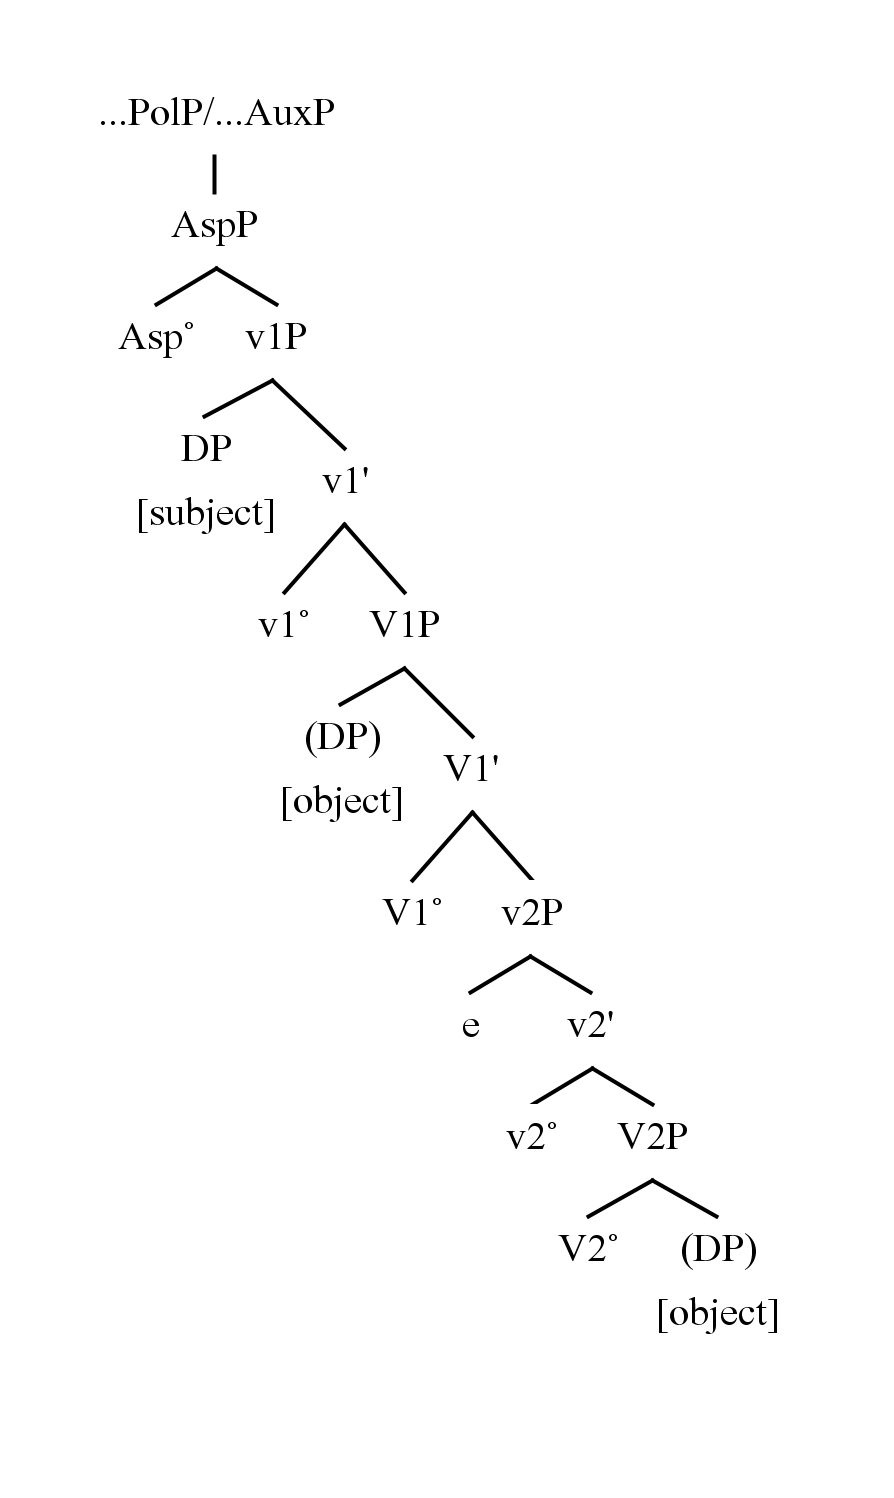
\includegraphics[width=\textwidth]{Rolle-img1.png}
\textbf{Figure }\textbf{: Degema SVC Syntax}
\end{figure}

In this structure, the second verb phrase (\textit{v}\textsubscript{2}P) is the complement of the first lexical verb (V1) (they are structurally adjacent and therefore sisters). To illustrate, consider the data from \citet{Collins1997} in \REF{ex:rolle:20}, from Ewe. Here, the second verb \textit{ɖu }‘eat’ is the complement of the first verb\textit{ ɖa }‘cook’. Note that surface word order is accounted for through syntactic movement.

\ea
\langinfo{Ewe}{}{}\\
\gll  M-a  ɖa    nu    ɖu\\
     I-\textsc{fut}  cook  thing  eat\\
\glt ‘I will cook something and eat it.’ \citep[490-491]{Collins1997}
\z

For reasons of space, we do not compare Collins’ proposal here to other syntactic analyses of SVCs (e.g. Baker 1989; Hiraiwa \& Bodomo 2008; Aboh 2009; among others). 

With respect to Degema clitics, we adopt that tense/aspect enclitics are in a functional head Asp(ect)° which selects a \textit{v}P as its complement. Functional heads such as Asp° take scope over both verb phrases. Note that although the position of Asp° is above the first verb, as enclitics they will appear after the verb(s). Further, subject agreement proclitics have no designated position in this syntactic structure. We follow \citet{EmbickNoyer2007}, \citet{Kramer2010}, \citet{Norris2014}, among others that agreement features are inserted post-syntactically, and therefore these clitics are purely morphological with no unique syntactic correspondent. 

\section{Arguments against the verb compound hypothesis}
\label{bkm:Ref449523633}
With this structure in mind, we can begin to account for the distribution of the clitic SVC patterns. As mentioned above, one possibility is to consider the Single-Marked Pattern as a verb compound, forming one syntactic constituent. One articulated theory within the generative tradition is Collins’ (2002) account of ǂHoan verb compounds. An example is provided in \REF{ex:rolle:21} where the two verbs in bold are contiguous, and marked only once by inflectional \textit{a- }\textsc{prog}.

\ea
\langinfo{ǂHoan}{}{}\\
\gll  Ma  a-\textbf{qǁhu    {\textbar}’o}    djo    ki      kx’u    na\\
     \textsc{1sg}   \textsc{prog}{}-\textbf{pour}  \textbf{put.in}  water  \textsc{particle}  pot    in\\
\glt ‘I am pouring water into the pot.’ \citep[1]{Collins2002}
\z

Under this analysis, the syntactic structure is largely identical to that adopted in 1 above involving nested VPs, in which the second verb phrase (\textit{v}\textsubscript{2}P) is the complement of the first lexical verb (V1). The critical parametric difference is that in ǂHoan the two verbs both undergo syntactic head-movement to a higher functional position (\textit{v}\textsubscript{1}°), and together form a complex head. We refer to this as the \textit{verb compound hypothesis}. Under this approach, we could capture the SVC patterns differences by saying that the Single-Marked Pattern is a verb compound exhibiting verb movement forming a complex head, whereas the Double-Marked Pattern exhibits no such movement. 

We present two arguments against the verb movement hypothesis. The first argument is that under the verb compound hypothesis there is unmotivated “blocking” of V2 movement to form a verb compound when there is an intervening object. As described above, the Single-Marked SVC Pattern occurs in Degema only if the structure consists of two adjacent verbs, or if there is a prosodically light intervening object. If there is a prosodically heavy intervening object, the two verbs exhibit the Double-Marked Pattern. Under the verb compound hypothesis, both verbs would undergo verb movement and form a complex head. Because this movement is head-movement, it would be unclear why the presence of an object in the V\textsubscript{1}P would block head-movement of V\textsubscript{2}° to \textit{v}°, but allow movement of V\textsubscript{1}°.

Specifically, under the verb compounding analysis we would expect the intransitive V\textsubscript{2} verb \textit{tạ }‘go’ to undergo head movement and form a complex verb compound with V\textsubscript{1} \textit{ḍuw} ‘follow’ in \REF{ex:rolle:22}. However, (b) below shows that this is ungrammatical. Example \REF{ex:rolle:23} shows it is equally ungrammatical for two transitive verbs to form a verb compound when an object is present. 

\ea
{Transitive + Intransitive}\\
\gll   Breno   o=ḍúw    mé   \textbf{tạ́}=\={a}n\\
     Breno   3\textsc{sg}=follow   me   \textbf{go}=\textsc{fe}\\
\glt ‘Breno went with me’ \citep[115]{Kari2004}
\z




\ea
  *Breno o=ḍúw  \textbf{tạ́}  mé=\={e}n\\
\z

\ea
{Transitive + Transitive (shared object)}\\
\gll   Jzakume   ọ́=tam      ị́ḍíyom  ọ=\textbf{ḍóny}\\
     Jzakume  \textsc{neg{\textbackslash}}3\textsc{sg}=chew  food  3\textsc{sg}=\textbf{swallow}\\
\glt Jzakume did not chew food (and did not) swallow’ \citep[110]{Kari2004}
\z




\ea
   *Jzakume  ọ́=tam  \textbf{ḍọny  }ị́ḍíyom\\
\z


In other verb compounding languages, the presence of an object also does not block verb compounding, e.g. Ju{\textbar}’hoan \citep{Collins2002}, Khwe (Kilian-Hatz 2006), Igbo \citep{Lord1975}, Isu (Kießling 2011), Toqabaqita (Lichtenberk 2006, 2008), and Eastern Kayah Li \citep{Solnit2006}. Noting that V2 in the examples above does not undergo head movement, these data cast doubt on the head movement analysis as a whole.

A second argument against the verb compound hypothesis is that the Single-Marked Pattern is found whenever the verbs are not separated by a prosodically heavy object. In many examples this happens when the first verb is intransitive, though it also is found when V\textsubscript{1} is transitive but the verb does not appear surface-adjacent to its syntactic argument. This can be seen in three circumstances: in object dislocation \REF{ex:rolle:24} (both content questions (24a-b) and focus constructions \REF{ex:rolle:24c}), object-drop, i.e. where the object of the verb simply has no overt phonological instantiation (marked in the examples by an underscore) \REF{ex:rolle:25}, and object relative clauses \REF{ex:rolle:26}. In each of these types, the transitive verb does not appear adjacent to its argument, and consequently appears surface-adjacent to the second verb in the SVC. Under these circumstances, a Single-Marked Pattern occurs.

\ea
{Dislocation of objects}\\
\gll   \textbf{Mi}=ḍúw=\textbf{n }    ovo     \textbf{mị}=tá=\textbf{\={a}n}\\
      \textbf{1}\textbf{\textsc{sg}}=follow=\textbf{\textsc{fe}}   who   \textbf{1}\textbf{\textsc{sg}}=go=\textbf{\textsc{fe}}\\
\glt ‘I went with who?’
\z

\ea
\gll   Ovó   nụ́   \textbf{mi}=ḍúw    Ø  tạ́=\textbf{\={a}n}\\
      who   that   \textbf{1}\textbf{\textsc{sg}}=follow     go=\textbf{\textsc{fe}}\\
\glt ‘Who did I go with?’
\z

\ea
    *Ovó nụ́ \textbf{mi}=ḍú\textbf{\={u}w} Ø \textbf{mị}=tá=\textbf{\={a}n}?\\
\glt ‘Who did I go with?’
\z

\ea
\gll   kụ́   ọ́yi     nụ     \textbf{mi}=ḍúw   \textbf{Ø}  tạ́=\textbf{\={a}n}\\
       not   her/him   that     \textbf{\textsc{1sg}}=follow     go=\textbf{\textsc{fe}}\\
\glt ‘It was not her/him that I went with’ 
\z

\ea
{Object-drop}\\
\gll  Ohoso   \textbf{ọ}=tá   ḍẹ́     vọ́     yị́    kị́yé=\textbf{n }  ọ́yi\\
     Ohoso   \textbf{3}\textbf{\textsc{sg}}=go   buy   \_\_  take \_\_  come   give=\textbf{\textsc{fe}}  her/him  \_\_\\
\glt ‘Ohoso went and bought (something) and brought (it) to her/him’ \citep[121]{Kari2004}
\z

\ea
{Relative clauses }\\
\gll  owéy     nụ́     \textbf{mi}=ḍúw Ø tá=\textbf{t\={e}}\\
     person    that    \textbf{\textsc{1sg}}=follow    go=\textbf{\textsc{prf}}\\
\glt ‘the person whom I have gone with’
\z

These data highlight that there is no strict association between clitic patterns and the argument structure of verbs in a SVC, but rather surfaces whenever the verbs are sufficiently local on the surface. 

\section{Phonological alignment of clitics }

We have argued above that appealing to syntactic structure and operations alone is insufficient to account for the distribution of inflectional clitics within SVCs in Degema. We therefore understand post-syntactic operations to play a major role in this distribution (assuming morphological and phonological modules containing such post-syntactic operations follow syntax). This will account for why different clitic patterns surface depending largely on how local the verbs are, and why prosodically light pronouns may intervene between the verbs in a Single-Marked Pattern. 

Recall from \sectref{sec:rolle:3.1} that we assume tense/aspect enclitics are in a high functional Asp° projection above the verb phrases, but that subject agreement proclitics are inserted post-syntactically. Regardless of the origin of these clitics, we must account for how the clitics appear in their surface position. We adopt what we call the \textit{clitic alignment hypothesis}, defined below. 

\section{\textit{Clitic alignment hypothesis}: For \textit{every} clitic and \textit{every} verbal host within a clause, align the clitic with the verbal host}

This principle states that there must be alignment between verbs and clitics within a clause, which takes place post-syntactically. Subject agreement proclitics are pre-specified as attaching to the left-edge, and tense/aspect enclitics to the right-edge. In the Double-Marked Pattern, because there are two verbal hosts in the clause, to satisfy this principle of alignment the clitics must align with both verbs, resulting in doubling of the clitics. 

In contrast, in the Single-Marked Pattern proclitics are only found on V1 and enclitics only on V2, which seemingly violates this hypothesis. However, if we understand that verbs which are linearly adjacent can form a single verbal complex and that clitics align to this complex, then these structures do adhere to the clitic alignment hypothesis. Under this hypothesis, verbal hosts can be either simplex verbs or complex verb clusters.

  A number of aspects of this hypothesis need to be fleshed out. One is which mechanism moves clitics from their original positions, tying to a rich literature on the nature and ontological status of post-syntactic movement, e.g. \citet{NesporVogel1986}, Bošković (2001), Anderson’s (2005) principles of \textit{stray adjunction }and\textit{ full interpretation}, mobile morphology in \citet{JenksRose2015}, among others. A second aspect is how we can get clitics to “copy” in the Double-Marked Pattern, a type of verbal concord. We cannot satisfactorily address these issues here, but we sketch below certain aspects of Degema grammar which support our hypothesis. 

One concerns the formation of a verbal complex resulting in the Single-Marked SVC Pattern. We presented evidence in \sectref{sec:rolle:3.2} that verbs showing a Single-Marked Pattern are not the result of syntactic movement and are not a verb compound, i.e. they do not form a syntactic constituent. We do, however, understand this verbal complex as forming a morphological constituent. \citet{Rolle2015} analyses the formation of constituents of verbs and clitics as due to the post-syntactic operation \textit{local dislocation }within Distributed Morphology (Embick \& Noyer 2001; 2007), which we adopt here. What is most important for our purposes here is that adjacent verbs form a single constituent (albeit not syntactically). 

With these assumptions we can account for the puzzling fact that prosodically light pronouns may intervene between verbs in the Single-Marked Pattern. We can think of the formation of the verb complex as sensitive to locality, but this locality is measured prosodically and not hierarchically. If the two verbs are separated by a prosodically heavy object, the verbs are not sufficiently local for the creation of the verbal complex, and therefore the Double-Marked Pattern results. If however we assume that monosyllabic pronouns are prosodically deficient – i.e. they do not project their own phonological word ($\omega $) –they are therefore transparent to the formation of the verbal complex. This is illustrated in \REF{ex:rolle:28} below, using data from the examples in \REF{ex:rolle:6} and \REF{ex:rolle:8} above. 

\ea
{Prosodically light pronouns         Prosodically heavy pronouns}
          \textsc{cl}=(        )=\textsc{cl}         \textsc{cl}=()=\textsc{cl   cl}=(  )=\textsc{cl}\\
     (\textsubscript{$\omega $}     )    (\textsubscript{$\omega $}   )  \textbf{Ø}   (\textsubscript{$\omega $}  )       (\textsubscript{$\omega $}    )        (\textsubscript{$\omega $}  )   \textbf{(}\textbf{\textsubscript{$\omega $}}  \textbf{)}  (\textsubscript{$\omega $}  )\\
     N      V    \textbf{$\sigma $}   V         N      V    \textbf{$\sigma \sigma $}    V\\
    Breno    ḍuw  \textbf{me}   tạ         Breno    ḍuw    \textbf{ọyi}    tạ\\
\z

We can understand this complex verb formation to be subject to inter-speaker variation and other complicating factors, which corresponds to the variation in the Single-Marked Pattern laid out in \sectref{sec:rolle:2.2.2.}

One might ask if the clitic alignment hypothesis is circular in the sense that we are defining morphological constituency based the distribution of clitics. Against this hypothesis, we find additional evidence for the constituency of the verbs in the verb complex in grammatical tone. In Degema, nouns are lexically contrastive for tone, but tone on verbs is determined solely by its grammatical context and not lexically specified. When verbs appear between a proclitic and an aspectual enclitic, all syllables are marked with high tone (H), shown in the Double-Marked Pattern in \REF{ex:rolle:29}.

\ea
{High tone pattern on verbs between clitics}\\
\gll  Tatane  o=\textbf{kótú}=té     éni   ọ=\textbf{kpérí}=t\={e}     ínúm\\
     Tatane  3\textsc{sg}=\textbf{call}=\textsc{prf}   us   3\textsc{sg}=\textbf{tell}=\textsc{prf}  something\\
\glt ‘Tatane has called us and told (us) something’ \citep[285]{Kari2003a} 
\z

This high tone pattern is also seen in verbal complexes with a Single-Marked Pattern, shown in \REF{ex:rolle:30}. In these cases, all words between the clitics are marked with high tone. 


\ea
{High tone pattern on verb complexes between clitics }\\
\gll   Ohoso   ọ=\textbf{tá  ḍẹ́    vọ́    yị    kịyé}=n   ọyi\\
     Ohoso    \textsc{3sg}=\textbf{go  buy    take  come  give}=\textsc{fe}   her/him\\
\glt ‘Ohoso went and bought (something) and brought (it) to him/her’ \citep[121]{Kari2004}
\z

\ea
\gll   Breno   o=\textbf{ḍúw    mé   tạ́}=\={a}n\\
     Breno   3\textsc{sg}=\textbf{follow  me   go}=\textsc{fe}\\
\glt ‘Breno went with me’ \citep[115]{Kari2004}
\z

Further evidence comes from grammatical tone expressing negation. Sentential negation is realized tonally by a high-low (HL) pattern: a high tone falls on the proclitic, followed by low tone on the verb. In \REF{ex:rolle:31a}, the proclitic \textit{mí=} is marked with high tone, and the verb \textit{seneke} ‘think’ with low tone. (Note that the factative enclitic does not occur under negation.)

\ea
{HL negation tone with verb complexes }\\
\gll   mí\textbf{=seneke}      mụ́   ívom\\
     \textsc{neg{\textbackslash}1sg}\textbf{=think}    in   inside\\
\glt ‘I don’t think so’ \citep[32]{Kari2004}
\z

\ea
\gll   ó=\textbf{ḍeri       me}   kạbuló   ó=\textbf{meme     ḍị}   ị́ḍíyóm   yọ\\
     \textsc{neg{\textbackslash}3sg}=\textbf{know  me}    because   \textsc{neg{\textbackslash}3sg}=\textbf{agree   eat}   food   the\\
\glt ‘(S)he refused to eat the food because (s)he doesn’t know me’ \citep[45]{Kari2004}  
\z

In \REF{ex:rolle:31b}, this HL negation tone also applies when the verb appears with another verb or a prosodically light pronoun, both Single-Marked contexts. Here, all elements in the complex are marked with low tone. We can compare this with Double-Marked contexts when there is a prosodically heavy intervening object. In \REF{ex:rolle:32a}, the first verb and proclitic \textit{vọn} ‘take’ is marked with the HL negation pattern, whereas the second verb \textit{fịya} ‘cut’ is marked with H, outside of the scope of negative tone. Example \REF{ex:rolle:32b} illustrates that marking both verbs with HL negation is ungrammatical. 

\ea
{Negation tone in Double-Marked Pattern}\\
\gll   Osoabo   \textbf{ọ=von}       ẹ́lege   \textbf{ọ=fíyá}\\
     Osoabo   \textbf{\textsc{neg{\textbackslash}3sg}}\textbf{=take}   knife   \textbf{3}\textbf{\textsc{sg}}\textbf{=cut}\\
\glt ‘Osoabo did not use a knife to cut something’ \citep[111]{Kari2004}
\z

\ea
\gll   *Osoabo  \textbf{ọ́=von}       ẹ́lege   \textbf{ọ́=fiya}\\
     Osoabo   \textsc{neg{\textbackslash}3sg}=take   knife   \textsc{neg{\textbackslash}}3\textsc{sg}=cut\\
\z

We can capture these data by understanding the verbs under the Single-Marked Pattern as forming a morphophonological constituent, for both clitic distribution and grammatical tone scope.%
\footnote{We 
  note that the full tonology of Degema has not been worked out, and that certain counter-exceptions occur which we cannot account for at present (see Rolle 2015). For example, the tone of the object may affect the tone on verbs in SVCs as in the Single-Marked future tense example below. Here, V1 has high tone, but V2 has a downstepped high:

  \ea
  H - downstepped !H tone pattern on verbs in Single-Marked Pattern\\
  \gll mọ=\textbf{tá    ḍẹ }  ạḅí\\
  3\textsc{sg}=\textbf{go  buy }  books\\
  \glt ‘(S)he will go and buy books’ 
  \z 


  The object in this example is lexically LH \textit{ạḅí }/àɓɪ/ ‘books’, but is realized as HH \textit{ạ́ḅí}. If this object is modified by \textit{yọ} ‘the’, both verbs have high tone with no downstep: \textit{mọ=}\textbf{\textit{tá ḍẹ }}\textit{ạḅí yọ} ‘(S)he will go and buy the books’. 
}

\section{Conclusion}

We have shown that Degema exhibits two distinct clitic patterns in SVCs: a Double-Marked Pattern found when the verbs are separated by a prosodically heavy object, and a Single-Marked Pattern found when the verbs are not separated by an overt object, or are separated only by a prosodically light pronoun. We showed that although the Single-Marked Pattern superficially resembles verb compounds involving verb movement, there were two strong arguments against this position, and we therefore view these verbs as not forming a syntactic constituent. Instead, we view the verbs as forming a morphophonological complex subject to clitic alignment under a clitic alignment hypothesis. The formation of this verbal complex is subject to locality conditions defined linearly (not hierarchically), which we argued accounts for why prosodically light pronouns may intervene between verbs within the Single-Marked Pattern. We supported this analysis with evidence from grammatical tone scope, though note much more work is needed on Degema tone.

\section*{Acknowledgments}


We would like to thank Ohoso Kari, a native speaker of Degema, whom we consulted on some of these data. Of the Berkeley community, we would like to thank Peter Jenks, Line Mikkelsen, Sharon Inkelas, Larry Hyman, Daisy Rosenblum, Nico Baier, Zach O’Hagan, Florian Lionnet, and Herman Leung. Thanks also to the audience of ACAL46, ACAL46 editors Doris Payne and Mokaya Bosire, and the anonymous reviewers.


\section*{Abbreviations}

\begin{tabularx}{\textwidth}{XXXX}
\lsptoprule

{Gloss} & {Meaning} & {Gloss} & {Meaning}\\
{\scshape 1/2/3} & {Person marking} & {\scshape npm} & {Non-past }\\
{\scshape cl} & {Clitic} & {\scshape pl} & {Plural }\\
{\scshape fe} & {Factative tense/aspect} & {\scshape prf} & {Perfect }\\
{\scshape fut} & {Future} & {\scshape prog} & {Progressive}\\
{\scshape inaux} & {Inceptive non-imperative auxiliary} & {\scshape rps} & {Reciprocal }\\
{\scshape iter} & {Iterative} & {\scshape set1/set2} & {Set 1 or 2 pronouns}\\
{\scshape neg} & {Negative} & {\scshape sg} & {Singular }\\
{\scshape nie} & {Negative imperative} & {\scshape tns} & {Tense }\\
\lspbottomrule
\end{tabularx}
 


\begin{verbatim}%%move bib entries to  localbibliography.bib 


Kari, Ethelbert E. 2005. Degema subject markers: Are they prefixes or proclitics? Journal of West African Languages 32(1& 2). 13-20.




\end{verbatim}
 
\printbibliography[heading=subbibliography,notkeyword=this]

\end{document}